\documentclass[]{elsarticle} %review=doublespace preprint=single 5p=2 column
%%% Begin My package additions %%%%%%%%%%%%%%%%%%%
\usepackage[hyphens]{url}
\usepackage{lineno} % add
\providecommand{\tightlist}{%
  \setlength{\itemsep}{0pt}\setlength{\parskip}{0pt}}

\bibliographystyle{elsarticle-harv}
\biboptions{sort&compress} % For natbib
\usepackage{graphicx}
\usepackage{booktabs} % book-quality tables
%% Redefines the elsarticle footer
%\makeatletter
%\def\ps@pprintTitle{%
% \let\@oddhead\@empty
% \let\@evenhead\@empty
% \def\@oddfoot{\it \hfill\today}%
% \let\@evenfoot\@oddfoot}
%\makeatother

% A modified page layout
\textwidth 6.75in
\oddsidemargin -0.15in
\evensidemargin -0.15in
\textheight 9in
\topmargin -0.5in
%%%%%%%%%%%%%%%% end my additions to header

\usepackage[T1]{fontenc}
\usepackage{lmodern}
\usepackage{amssymb,amsmath}
\usepackage{ifxetex,ifluatex}
\usepackage{fixltx2e} % provides \textsubscript
% use upquote if available, for straight quotes in verbatim environments
\IfFileExists{upquote.sty}{\usepackage{upquote}}{}
\ifnum 0\ifxetex 1\fi\ifluatex 1\fi=0 % if pdftex
  \usepackage[utf8]{inputenc}
\else % if luatex or xelatex
  \usepackage{fontspec}
  \ifxetex
    \usepackage{xltxtra,xunicode}
  \fi
  \defaultfontfeatures{Mapping=tex-text,Scale=MatchLowercase}
  \newcommand{\euro}{€}
\fi
% use microtype if available
\IfFileExists{microtype.sty}{\usepackage{microtype}}{}
\usepackage{graphicx}
% We will generate all images so they have a width \maxwidth. This means
% that they will get their normal width if they fit onto the page, but
% are scaled down if they would overflow the margins.
\makeatletter
\def\maxwidth{\ifdim\Gin@nat@width>\linewidth\linewidth
\else\Gin@nat@width\fi}
\makeatother
\let\Oldincludegraphics\includegraphics
\renewcommand{\includegraphics}[1]{\Oldincludegraphics[width=\maxwidth]{#1}}
\ifxetex
  \usepackage[setpagesize=false, % page size defined by xetex
              unicode=false, % unicode breaks when used with xetex
              xetex]{hyperref}
\else
  \usepackage[unicode=true]{hyperref}
\fi
\hypersetup{breaklinks=true,
            bookmarks=true,
            pdfauthor={},
            pdftitle={Predictive Models to Support Quoting of Fixed Fee Consulting Projects},
            colorlinks=true,
            urlcolor=blue,
            linkcolor=magenta,
            pdfborder={0 0 0}}
\urlstyle{same}  % don't use monospace font for urls
\setlength{\parindent}{0pt}
\setlength{\parskip}{6pt plus 2pt minus 1pt}
\setlength{\emergencystretch}{3em}  % prevent overfull lines
\setcounter{secnumdepth}{0}
% Pandoc toggle for numbering sections (defaults to be off)
\setcounter{secnumdepth}{0}
% Pandoc header


\usepackage[nomarkers]{endfloat}

\begin{document}
\begin{frontmatter}

  \title{Predictive Models to Support Quoting of Fixed Fee Consulting Projects}
    \author[Queensland University of Technology]{Amy Cook, Paul Wu, Kerrie Mengersen\corref{c1}}
   \ead{a21.cook@qut.edu.au} 
   \cortext[c1]{Corresponding Author}
      \address[Queensland University of Technology]{School of Mathematical Sciences, George Street, Brisbane, QLD, 4000}
  
  \begin{abstract}
  A concise abstract is required. limit to 250 words. clearly state
  purpose of research, principal resutls and major conclusions. no refs
  
  Engaging in loss making jobs for fixed fees is a major problem in
  consulting, particularly in the competitive construction industry. This
  thesis investigates whether machine learning techniques applied to a
  company's passively collected internal data could help avoid loss making
  jobs or help tactfully choose when to enforce stricter contracts. It was
  found that in a specific decision framework, a case study's profits
  could be improved 9\% by declining approximately 4\% of projects.
  Alternative decision frameworks are also proposed and evaluated.
  Algorithmic methods such as Logistic Regression, Random Forests, Boosted
  Trees, Naive Bayes, and Bayesian Networks were applied as well as
  blended combinations of these methods. A decision scenario which
  rejected projects above a sequence of tested thresholds was run in order
  to find the optimal threshold for profit improvements. The blended
  Logistic Regression model outperformed other methods and produced a 95\%
  confidence interval of 6.5 - 11.5\% profit improvements. The findings
  from this research have the potential to assist managers in reducing
  losses by highlighting risky projects and guiding project-based changes
  to fee structures.
  \end{abstract}
   \begin{keyword} consulting; machine learning; profitability; predictive model;
construction industry; data mining \sep \end{keyword}
 \end{frontmatter}

\emph{Text based on elsarticle sample manuscript, see
\url{http://www.elsevier.com/author-schemas/latex-instructions\#elsarticle}}

\section{1. Introduction}\label{introduction}

Clearly state the research question and objectives of the work. Briefly
provide any necessary background to frame the research question.
Concisely summarize the major findings/results.

Many consulting projects can be financialy risky endeavors for the
consultant, often depending on the industry. Engineering consultanting
companies in the construction industry complete a wide range of complex
projects in a competitive enviroment. Because of the way contracts are
structured, many of these projects result in losses. The purpose of this
study was to test whether these loss making projects could be predicted
by statistical and machine learning algorithms using the information
available at project conception. Secondly, could the predictive
algorithm improve a company's profitability? Predictive models and value
frameworks were built using project data from a case study engineering
company to answer these questions.

1 page

\paragraph{1.1 Problem motivation}\label{problem-motivation}

Financial risk is taken on by a consulting company when they offer a
fixed fee to complete a project. In competitive climates, clients are in
the position to request fixed price quotes from several consultants
before a project is awarded. Hence, initial quoted fees must be
competitive but also accurately cover consultant salaries and business
costs.

How do consultants make this accurate yet competitive fee estimate? This
varies from industry to industry, but typically a consulting manager has
experience in the type of project they are quoting and, after reviewing
the project details, can use a combination of intuition, analysis of
project details, and rules of thumb. Unfortunately, some projects priced
using this method can blow out of budget, causing significant financial
losses to the consultant.

Cost blowouts of complex projects has a history, particularly documented
in the It and construction industry. A review of 6 IT project surveys
between 1984 and 1994 by Moløkken \& Jørgensen (2003) revealed that
60-80\% of IT projects encountered effort and/or schedule overruns,
where the average overrun was by 30 to 40\%. A study on large-scale
infrastructure projects over the past seventy years revealed that cost
forecasts consistently underestimated the cost of rail projects by an
average of 44.7\%, the cost of bridge and tunnel projects by 33.8\% and
the cost of road projects by 20.4\% (Flyvbjerg 2007).

Kahneman won a nobel prize in 2002 for his research into decision making
on this topic. He argued that a person's natural optimistic view of
their own skills leads to consistent underestimation of the time and
risks involved in a project (Lovallo and Kahneman 2003). To counter this
phenomenon, research by Flyvbjerg {[}-Flyvbjerg2011{]} advised that
managers should be confronted by the financial performance of similar
projects to the one being costed so that they take on a more realistic
view of their abilities. This was based off a body of findings where
people made better predictions about themselves after being exposed to
facts about other people. For example, subjects were asked to predict
their skill levels before and after being exposed to a summary of other
people's skills, and their predictions after were significantly more
accurate (Lovallo and Kahneman 2003).

This work aims to help managers provide better fixed price quotes by
predicting whether a new project will be profitable or not, based on an
algorithm trained on all previous project data from the same company.
The manager could take multiple actions based on the algorithms output
including not tendering for a project predicted to be loss-making,
providing a high fixed price, or restructuring the contract so that it
is not 100\% fixed price. This research tests the simple case of
rejecting all projects predicted as loss-making.

\paragraph{1.2 Case Study}\label{case-study}

Project data from a single case study consulting company in the
construction industry was used to build the predictive algorithm, trial
several methods, and test their impact on the company's bottom line.
Twelve years of passively collected data that described each project in
terms of their clients, invoice history, employee hours and technical
details was scraped from the company's internal database. Customer
relationship management (CRM) software provided accesses to the database
to all employees. Employees completed daily timesheets, alotting their
hours to certian projects. Project managers input technical information
and client details for each project, while the finance team tracked
invoicing and additional project costs such as printing and transport in
the same system. On top of this information, the CRM had the hourly cost
of each level of employee. The cleaned dataset consisted of 2364
projects between 2004 and 2012. 70\% of projects were fixed price and
20\% of all projects made a loss after taking into account business
costs.

Once several methods were built, to assess whether the model would
improve the case study company's profitability, a simple managerial
decision framework was applied: if the algorithm predicted the project
to be loss making, the project was considered `rejected' and all profits
or \emph{losses} of rejected projects were discarded. The remaining
projects' profits and losses were summed to give a revised overall
profit over the last 12 years of projects. This was compared to the
summed profits and losses from all projects completed over the last 12
years. The best algorithm rejected enough loss-making projects to
improve overall profits by 9\%.

\section{2. Literature Review}\label{literature-review}

For the case study company, training the algorithm to predict actual fee
was not possible because the projects were too varied, and there was
inadequate information describing the size and scope of each project in
the database. However, in the literature, similar studies typically did
attempmt to predict project costs of IT consutling projects and final
construction costs of buildings and infrastructure.

\paragraph{2.1 Cost estimation in the Construction Industry and IT
Industry}\label{cost-estimation-in-the-construction-industry-and-it-industry}

Previous studies in the literature have focussed on reporting the
predictive accuracy of their cost estimation models for IT or
construction projects using data from multiple businesses or governments
around the world. In contrast, this research is focussed on determining
how or if models predicting project profitability can improve the bottom
line for a case study business, given data the company has internally
generated.

Reviewing a range of individual studies show that cost estimation models
have generally been built from at most 530 projects (Kim, An, and Kang
2004) (Finnie, Wittig, and Desharnais 1997) - 299 software
development(Pai, McFall, and Subramanian 2013) - 163 software (Shin
2015) - 234 building projects, and often under 100 projects (Finnie,
Wittig, and Desharnais 1997) (Chan and Park 2005) 87 buildings.
Sometimes it is not stated where the project data came from, and some
studies specified the information came from surveys, with responses from
companies and governments around the world. In this study, the dataset
originates from a single company's database, which means the data is
easily accessible to the company and there are 2364 projects, which is
much more than previous studies. A study by Mendes and Kitchenham (2004)
demonstrated that using within company data was also more accurate than
across company data. Their dataset consisted of 67 across company web
projects and 14 within company projects.

Almost all past studies analysed their model performance by predictive
accuracy (reported as R\^{}2 or RMSE) of cost predictions
({\textbf{???}} some stff) and compared these statistics bewteen
methods. However, these results were not translated into a business case
for the impact these models could have on an institution or how the
model could be practically integrated into decision making. For example,
if an institution used the model, how would it be applied to their
decision making process and what magnitude of benefits could they
expect? Saradhi \& Palshikar's (2011) work on employee churn, where
`churn' refers to the number of individuals moving out of a group within
a certain time, presented a good framework for implementing their model.
Theirsupport vector machine (SVM) predictive model identified employees
at high risk of churn. Then a method for determining the value of each
employee in terms of their importance to projects and their monthly
chargeability was described, which enabled high risk employees to be
ranked. Managers then had a clear direction for who to target first to
prevent churn. This extension provided a comprehensive framework for how
business managers could adopt a machine learning algorithm to improve
business operations. It was a valuable addition that is absent from most
cost estimation research, but will be included in this work.

\paragraph{2.2 Methods used in Cost Estimation and Other Business
Applications}\label{methods-used-in-cost-estimation-and-other-business-applications}

Cost estimation literature tended to apply linear regression, neural
networks and sometimes SVM methods, while predictive methods applied to
other business problems investigated a wider range. This study aims to
compare a wider range of methods to past cost estimation studies.

In the construction industry, often only one method was assessed, such
as linear regression, without comparison to other methods (Chan and Park
2005; Elfaki, Alatawi, and Abushandi 2014). Neural Networks started
appearing in literature in the 1990's and Elfaki, Alatawi, and Abushandi
(2014)`s review of cost estimation methods from 2004 to 2014 found that
artificial Neural Networks and SVM's were the most popular machine
learning techniques, but studies tended to only test one method. Some
studies showed that Neural Networks outperformed Linear Regression,
however other studies established they are approximately equal (Kim, An,
and Kang 2004; Attalla and Hegazy 2003). To the authors' knowledge Shin
(2015) documented the only application of ensemble tree methods (Boosted
Trees) to cost estimation in construction projects. They found Boosted
Trees slightly outperformed Neural Networks, but not significanatly.

In the software cost estimation literature, Linear Regression was the
most popular method, however multiple studies showed that Neural
Networks definitively outperform regression models (Finnie, Wittig, and
Desharnais 1997; Pai, McFall, and Subramanian 2013; Matson and
Mellichamp 1993). Despite the higher performance, Neural Networks were
criticised for not providing reasoning or structure behind their
predictions (black-box predictor) (Finnie, Wittig, and Desharnais 1997).

The review of methods applied to the construction and IT industry
highlighted the use of Linear Regression, Neural Networks, SVM's and in
one case Boosted Trees, however research on other business problems
utilised a wider range of methods. In financial credit scoring, a study
by Brown and Mues (2012) found that Random Forests and Boosted Trees
consistently outperformed Neural Networks in classification. In
addition, ensemble trees such as Random Forests and Boosted Trees can
output partial dependency plots and variable importance measures that
provide insight into the model's calculations. This is a valuable asset
oer black box predictors. Kumar and Ravi (2007) performed a detailed
review of statistical and machine learning techniques applied over 37
years in the context of bankruptcy prediction in banks and reported that
although SVM's performed well, they are often complex and slow,
requiring a great deal of memory. They also assessed method blending
techniques, which refers to combinations of two completely different
algorithms, and found they can often outperform individual methods such
as Linear Regression or Boosted Trees alone.

To date, Linear Regression, Neural Networks, and Support Vector Machines
(SVM's) have been comprehensively applied to cost estimation. This
research does not test black-box predictors (Neural Networks and SVM's)
because insight into the model's predictions is crucial for facilitating
user uptake in the case study company. Ensemble tree methods such as
Random Forests and Boosted Trees will be used instead, as they can
perform as well as Neural Networks while providing insight to their
output (Caruana and Niculescu-Mizil 2006). Blending of multiple
predictive models is also applied in this work and has not yet been done
in cost estimation.

\paragraph{2.3 Gaps}\label{gaps}

In comparison to previous studies, this project advances the body of
work on cost estimation in two ways. First, it focusses on building a
model that is practical and profitable for a business to implement by
using the case study's interenal database as well as testing a
managerial decision framework based off the model output. This framework
presents a clear measure of expected benefits provided by adopting the
profitability model into a business' decision process. Secondly,
advanced predictive methods are trialled which have been minimally
tested on this problem. These include ensemble decision tree methods,
such as Random Forests and Boosted Trees, and blends of multiple models
built from different methods.

\section{3. Prediction Methods}\label{prediction-methods}

Should provide sufficient detail to allow the work to be reproduced.
Methods already published should be indicated by a reference: only
relevant method modifications should be described.

A range of simple and complex, linear and non-linear methods were
applied to the problem including Logistic Regression, Random Forests,
Gradient Boosted Trees, and Naiive Bayes. Furthermore, logistic
regression, random forests, boosted trees and simple averaging were used
to blend predictions from individual models. A brief description of each
method is provided below.

\paragraph{3.1 Predictive methods}\label{predictive-methods}

The aim of this research is to build a model that predicts whether a
consulting project will be profitable or not. Therefore each method must
be capable of binary classifcation. Binary classification output from a
model is the probability, between 0 and 1, of an event occuring. In this
case, the event is a project being loss-making.

\subparagraph{3.1.1 Logistic Regression}\label{logistic-regression}

Logisitic regression models a linear relationship bewteen the log odds
of a binary response variable and each of the explanatory variables.
This is performed similarly to linear regression, but is transformed to
probability of an event occuring by taking the inverse log of the log
odds and rearranging (Macdonald 1975):

\[
\begin{aligned}
\log(odds) &= \beta_0 + X_1\beta_1 \\
\log\left(\frac{p}{1-p}\right) &= \beta_0 + X_1\beta_1 \\
-\log\left(\frac{1-p}{p}\right) &= \beta_0 + X_1\beta_1 \\
-\log\left(\frac{1}{p} - 1\right) &= \beta_0 + X_1\beta_1 \\
\log\left(\frac{1}{p} - 1\right) &= -\beta_0 - X_1\beta_1 \\
\exp\left(\log\left(\frac{1}{p} - 1\right)\right) &= \exp(-\beta_0 - X_1\beta_1) \\
\frac{1}{p} - 1 &= \exp(-\beta_0 - X_1\beta_1) \\
\frac{1}{p} &= 1 + \exp(-\beta_0 - X_1\beta_1) \\
p &= \frac{1}{1 + \exp(-\beta_0 - X_1\beta_1)}
\end{aligned}
\]

The result in a sigmoidal function bound by 0 and 1. A coefficient
represents the change in the log odds of the response variable for each
unit increase in an explanatory variable. Logistic Regression is a good
benchmark to compare other binary predictive models due to its
simplicity and speed (Moore and McCabe 1989). Addittionally, because of
the simple, single linear relationship, the method is not prone to
overfitting (Perlich, Provost, and Simonoff 2003).

\subparagraph{3.1.2 Random Forests}\label{random-forests}

Ensemble tree methods were pioneered in the 1990's to combat the low
predictive accuracy and instability of individual decision trees.
Combining hundreds or thousands of trees transform decision trees into
high performing, stable predictors (Breiman 1996).

The Random Forests algorithm works by training multiple trees from the
bootstrapped samples of a dataset. Additionally, when creating each
tree, a random subset of attributes (covariates) is considered at each
split. The reduced subset of covariates is resampled for each split in
the tree. Dominant covariates are then suppressed for a fraction of the
splits, allowing the algorithm to explore signals in weaker covariates
(Breiman 2001). Performance statistics and tests run within the
algorithm provide insights to the modeller, such as variable importance
and variable relationships (Sealfon and Gymrek 2012).

\subparagraph{3.1.3 Gradient Boosted
Trees}\label{gradient-boosted-trees}

The boosted decision tree approach applies gradient descent theory to a
series of decision trees. Performance tends to be higher if individual
trees are limited to a certain depth to maintain simplicity and prevent
overfitting (Elith, Leathwick, and Hastie 2008). Unlike Random Forests,
the trees are sequential, where each tree models the residuals (or
errors) of the preceding tree.

By modeling the errors, misclassified cases are weighted higher than
correctly classified cases and influence the structure of the next tree
more (Hastie, Tibshirani, and Friedman 2009). This increased weighting
of error cases is called boosting. The successive results of up to
thousands of trees is very powerful (Elith, Leathwick, and Hastie 2008).
Caruana and Niculescu-Mizil (2006) tested Boosted Trees, Random Forests,
Neural Networks, SVM's, Logistic Regression and Naive Bayes on 11 binary
classification problems and found that Boosted Trees performed best,
followed by Random Forests. This demonstrates how capable ensemble tree
methods are of competing with high-level machine learning algorithms.

\subparagraph{3.1.4 Naive Bayes}\label{naive-bayes}

Naive Bayes is a simple, fast method included in this work because,
similarly to Logistic Regression, it provides a good baseline method
against which to compare complex methods (Caruana and Niculescu-Mizil
2006). It works by making conditional independence assumptions about the
explanatory variables in order to simplify probability calculations for
a categorical response variable. For example, if predicting a binary
variable, \(R\) (with classes 0 or 1) given two covariates \(X_1\) and
\(X_2\), the equations for the probability of both outcomes is as
follows:

\(p(R = 1|X_1 X_2) = p(X_1|R = 1) \cdot p(X_2|R = 1) \cdot p(R = 1)\)

\(p(R = 0|X_1 X_2) = p(X_1|R = 0) \cdot p(X_2|R = 0) \cdot p(R = 0)\)

These equations are simple to compute given the data, and the class with
the highest probability can then be chosen (F. Provost and Fawcett
2013). The method can perform well in real world tasks because the
assumption of independence does not significantly damage predictions,
but amplifies the magnitude of the probability (F. Provost and Fawcett
2013). This is fine for ranking class 0 against 1 but the output
probabilities are not accurate statistical probabilities (Caruana and
Niculescu-Mizil 2006).

\subparagraph{3.1.5 Model Blending}\label{model-blending}

Several research groups involved in the high profile data science
competition, Netflix Prize, developed sophisticated methods of model
stacking, otherwise known as ensemble methods or model blending (Sill et
al. 2009). In this paper, the term `blending' will be used to avoid
confusion with ensemble tree methods. Model blending combines
predictions from several models that used methods with different
theoretical foundations. In this way, the strengths of each method can
be combined. Since the 1990's research in statistics has shown that
averaging results from different methods can provide better predictive
accuracy than any single model (Madigan and Raftery 1994).

Six blending methods, ranging from simple to complex, were chosen. These
included simple averaging of the individual model results, building a
Logistic Regression model and Boosted Tree model using individual model
results only, feature weighted linear stacking (FWLS), Random Forests,
and Boosted Trees. The first two models are simply the average, and
weighted average of predictions from separate individual models. For
example, if the Logistic Regression model output a probability of 0.6
for one case, while a Boosted Tree output 0.7, a simple blended average
for that case would be a probability of 0.65. The last three methods are
more complex, and take advantage of potentially meaningful interactions
between the individual model predictions and the original covariates
describing each case (called meta-features in the model blending
literature) (Sill et al. 2009). For example, if the Logistic Regression
model predicted profitability better than the Boosted Tree model for
projects with only one team member, the complex blending methods would
take advantage of this interaction. In summary, in the complex methods,
the probability outputs from each model are interacted with each of the
original covariates. Model blending has the potential to elevate output
from the original methods by combining each of their strengths.

\paragraph{3.2 Procedure}\label{procedure}

The raw data from the case study company's database consisted of three
separate datasets: one describing the client and technical details for
each project, another with each employee's time sheet entries, and
another with all past invoices. This data was combined, cleaned, and
rearranged so that each project was described within one row. From the
timesheet data, 10 variables were engineered including the percent of
hours performed by `professional' employees as opposed to `technical'
employees, and the position of the employee that completed the most
hours on each project. 3 variables were engineered from the invoicing
data such as total amount invoiced for a project and mean invoice size
for a client. Finally, from the project dataset, 2 variables were
engineered including the number of projects completed with a client, and
project category. Text analysis of the project description determined
the project category variable. The response variable, whether the
project was profitable or not, was calculated by subtracting the cost of
employee hours from the timesheets from the sum of the paid invoices for
a project. The total amount invoiced for projects ranged from \$500 to
over \$1,000,000.

34 covariates made up the full dataset, and these were narrowed down to
11 in order to reduce predictive noise and provide a simple model that
is comprehendable for stakeholders (Weisberg 2005). Variable selection
methods included linear regression, random forests, and cforests and the
final variables are listed below.

\begin{itemize}
\tightlist
\item
  \% of Hours Completed by a Professional-level Employee
\item
  Time span
\item
  Number of Employees on Project
\item
  Amount Invoiced for Project
\item
  Business Category of Client
\item
  Project Category
\item
  Total Amount Invoiced from the Client - Past Jobs
\item
  Discipline
\item
  Position of Main Project Employee - new variable from ANOVA findings
\item
  \% of Hours by Main Project Employee
\item
  Billing Type
\end{itemize}

Timespan and the total amount invoiced are unknowns at before a project
commences. Therefore, these variables were discretised into 5 or 6
categories from which a manager would be able to select. The category
boundaries were determined by visualising clusters using hierarchical
dendrograms.

\subparagraph{3.2.1 Research Question 1}\label{research-question-1}

To answer the first research question, if loss making projects can be
predicted using statistical and machine learning algorithms, the binary
classification and blending methods were built and evaluated. The area
under the receiver operating characteristic (ROC) curve (AUC) statistic
was used to compare models and assess performance. Models were built on
a training subset of data (80\%) and validated on the remaining data.
Therefore, different training and testing sets produced different AUC
statistics. In order to compare which models performed significantly
better than others, an adequate sample size of AUC statistics was
required. A two-sample power calculation run on 20 AUC output for each
model determined that 100 samples were required to achieve a statistical
power of 0.8.

Then, the model output from the validation sets were combined and fed
into the three simple and three complex blending models. Again, 100
models were built to achieve a power of 0.8 for the variation in AUC
test statistics across different divisions of training/testing data. A
maximum of five training and validation divisions were created from a
complete set of individual model results.

\subparagraph{3.2.2 Research Question 2}\label{research-question-2}

The second research question asks whether a predictive algorithm can
improve a company's profitability. The model with the highest AUC score
may not improve company profits the most, because the magnitude of the
profits and losses from each project have not been analysed. Therefore,
all blended and individual models were carried forward to be assessed in
a value framework.

Once a model outputs scores for the probability of each job being
loss-making, the question then arises at what probability would a
manager round the probability up to 1? And then what action would be
taken? A threshold point between 0 and 1 can dictate when a project is
rounded up, and classified as `loss-making'. For this analysis, a simple
decision scenario is tested where a manager rejects all projects with
output above the threshold. For example, if the threshold is 0.6, and a
project is predicted to have a probability of loss-making of 0.7, the
project is rejected and profits or losses associated with the project
are ignored.

To test each threshold between 0 and 1, profit curves were built for
each method. This chart plots the probability threshold on the x-axis
and the ratio of model-influenced profits over historical company
profits on the y-axis. The ratio represented by the y-axis is calculated
using the formula below:

\[
\begin{aligned}
Ratio\ of\ Model\ Profit\ to\ Historical\ Profit\ (\%) &= \frac{\sum_{p = 1}^{N} I(Pr_p < threshold) \cdot Profit_p}{\sum_{p = 1}^{N} Profit_p} \cdot100
\end{aligned}
\]

Where

\[
\begin{aligned}
I(\cdot) &= \textrm{the indicator function} \\
N\ &= \textrm{the number of individual projects that are being included in the analysis} \\
Pr_{p} &= \textrm{probability output from the algorithm for project}\ p \textrm{. Values are}\\
& \qquad \textrm{betweeen 0 and 1 where 1 is loss making)} \\
threshold &= \textrm{a chosen value between 0 and 1.}\ \Delta\ Overall\ Profit\ \textrm{is calculated for} \\
& \qquad \textrm{several}\ threshold\ \textrm{values which defines the profit curve} \\
Profit_p &= \textrm{profit for individual project}\ p
\end{aligned}
\]

If the threshold were zero, all jobs were rejected, the profit would be
\$0, and the ratio to historical profits would be 0\%. If the threshold
was 1.0, all jobs were accepted and the profit would be the same as
historical profits, giving a ratio of 100\%. The total profits were
plotted for each threshold and joined to make a profit curve. The aim
was to find the optimal threshold point where mostly loss-making
projects were rejected, resulting in higher profits. 100 profit curves
were built for each method to achieve a power of 0.8 and a 95\%
confidence interval could also be determined around each threshold
point. The final expected increase in profit combined with the
percentage of projects to be rejected presents a clear scenario that the
case study business managers could strategically assess for
implementation.

\section{4. Prediction Results and
Discussion}\label{prediction-results-and-discussion}

Present results clearly and concisely discussion should explore the
signficance of the results of the work, not repeat them.

\paragraph{4.1 Individual Models}\label{individual-models}

The violin plot below summarises the distributions of the 100 AUC values
produced by each method. The `violins' are coloured according to whether
the distributions significantly vary to Boosted Trees using a critical
value of 0.05. Boosted Trees was chosen as the comparison method because
it was expected to perform well.

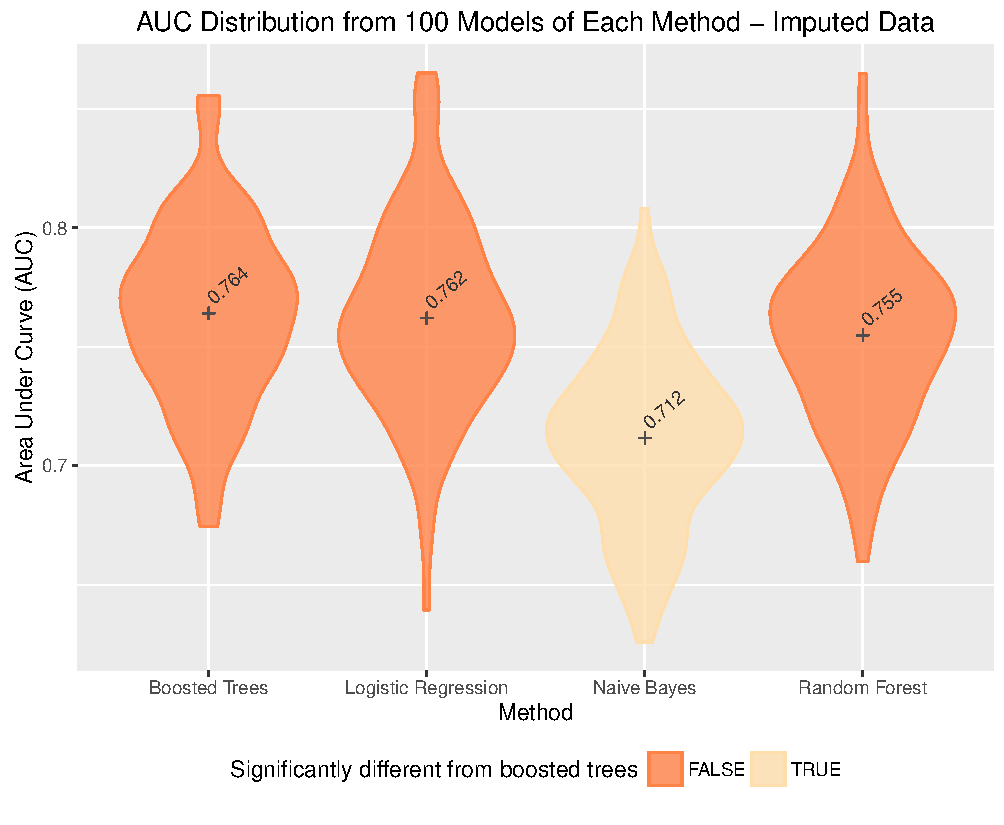
\includegraphics{Consulting_Profitability_Paper_files/figure-latex/mice_violin-1.pdf}

The AUC distrubtions of Logistic Regression and the Random Forest
algorithms could not be statistically differentiated from Boosted Trees,
while the Naive Bayes distribution was significantly lower. The three
high-performing methods had AUC values between 0.755 and 0.764. This
indicates predictions were well above random chance, where AUC = 0.5.

Naive Bayes and Logistic Regression were included as baseline models and
it was expected that the more complex models would outperform these.
Therefore it was surprising that results from 100 Logistic Regression
models were not statistically significantly lower than Boosted Trees. A
possible explanation for this, according to the literature, is that
there was not enough data for the ensemble trees to learn the complex
decision rules at which they excel. Trees tend to overfit the patterns
in a smaller training set. Logistic Regression on the other hand is
capable of only one decision boundary (which does not have to be
parallel to the variable axes) and is not prone to overfitting (Perlich,
Provost, and Simonoff 2003). This may explain Logistic Regression's
comparatively high performance on the case study's data set, which is
small for the range and complexity of the described projects.

\paragraph{4.2 Blended Models}\label{blended-models}

Six blended models combined the predictions from the three
high-performing individual models: Logistic Regression, Random Forests,
and Boosted Trees to create `blended' predictions. There were 3 simple
blended models, and 3 complex models that interacted original covariates
with the individual model predictions. Through variable importance
analysis on the original covariates and the 3 new variables containing
model predictions, only 6 original covariates were included as
metafeatures. All six blended methods' AUC values were compared against
the Logistic Regression AUC distribution, which was chosen because it
was the simplest high performing individual model.

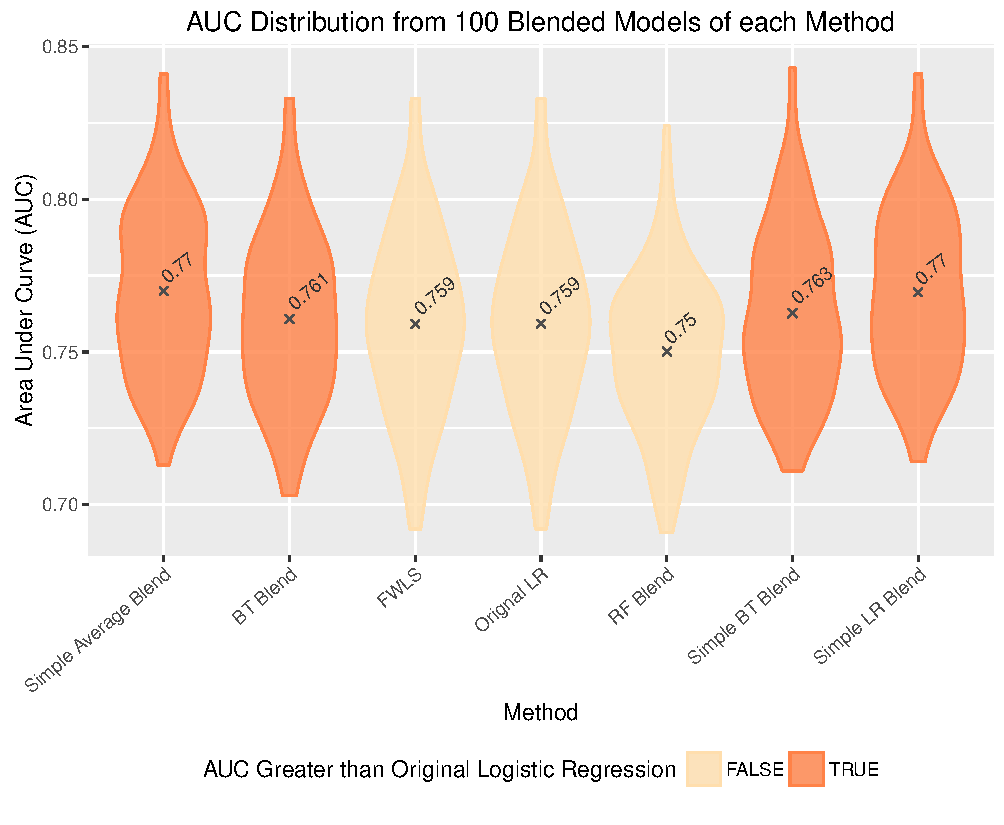
\includegraphics{Consulting_Profitability_Paper_files/figure-latex/blend_violin-1.pdf}

None of the blended methods were significantly higher than the
individual Logistic Regression model with data from 100 models. However,
the simple averaged method and simple logistic regression could achieve
a statistical power of 0.8 with 150 samples (models), whereas the other
blended methods required thousands. 50 more models were run for the
simple logistic regression and simple average blend to confirm their AUC
distributions were significantly higher than the individual Logistic
Regression. P-values from two sample t-test were 0.0019 and 0.0021
respectively.

Blended models improved the mean AUC from 0.759 to 0.77, which is an
increase of 1.4\%. This confirms the expectation that model blending
would improve predictions by combining the strengths of different
methods' theoretical foundations.

Again, the simplest methods worked best. In this case, averaging the
results of the best three individual models or taking a Logistic
Regression of the three models' outputs outperformed the complex Boosted
Trees, Random Forests, and Logistic Regression blends that facilitated
meta-feature interactions. Simiarly to the individual models, Simple
methods may outperform complex methods if the data is not big enough for
complex methods to learn the intricate patterns at which they excel. The
Netflix data set comprised of almost 3,000,000 observations, so the size
of the data could have enabled the success of their complex blending
methods (Feature Weighted Linear Stacking) (Sill et al. 2009)

The outcomes in this section show that statistical and machine learning
methods can predict whether a consulting project will be profitable or
not to some extent. The average, or weighted average (logistic
regression) blend of individual Logistic Regression, Boosted Trees, and
Random Forests models produced the highest AUC values. However, the
business value of the model has not been proven. The following section
explores whether the models would improve overall profits for the case
study business.

\section{5. Business Impact}\label{business-impact}

This chapter transports model results into the value framework to assess
impact on the case study's overall profitability. The plot below
illustrates the distribution of profit curves for the 100 models built
using each method. Solid lines join the mean values at each threshold
point and the grey ribbon represents the 95\% confidence interval for
the profit ratio.

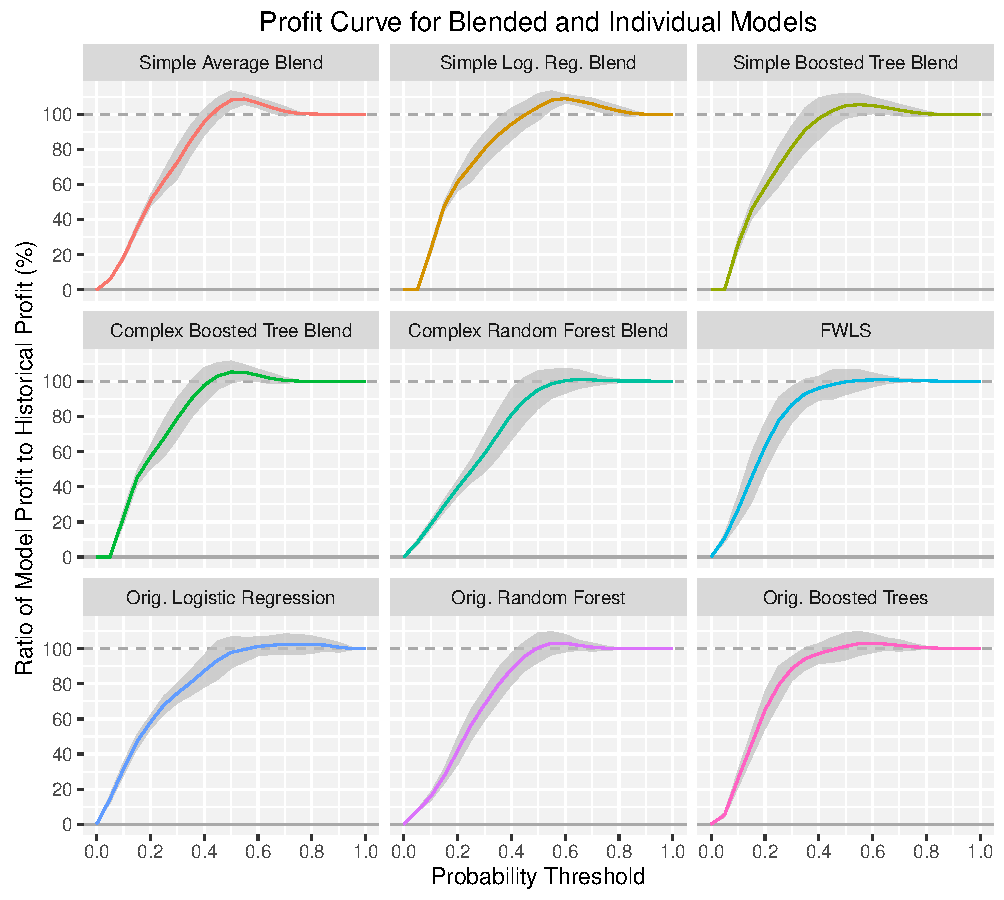
\includegraphics{Consulting_Profitability_Paper_files/figure-latex/profit_curve-1.pdf}

From the profit curves, the optimal probability thresholds are where the
profit curves peak, and peaks above 100\% indicate the model assisted
profits outperformed historical profits. The two simple blended models
clearly outperformed all other models with higher profit ratios as well
as tighter confidence intervals. The simple Logistic Regression blend
performed best with the highest mean profit ratio of 109\% and a
standard deviation of 1.28\%. This means that if all jobs above the
probability threshold 0.6 were rejected, the profits would increase on
average by 9\% in comparison to historical profits. Only 4.3\% of
projects were rejected in this case.

Profit curves from the simple blended models outperformed the complex
blended models, which follows logically from their significantly higher
AUC distributions. The shaded grey 95\% confidence intervals show that
none of the lower bounds for the original methods' or complex blending
methods were above 100\% on the y-axis. That is, it cannot be said with
95\% confidence that these methods would produce a mean profit higher
than historical profits in the given decision framework. It is
interesting that despite the reasonable AUC values, the profit curves
for the individual and complex blended models do not make a complelling
case for adoption into business practice.

The simple blended Logistic Regression model on the other hand, a mean
9\% improvement in profits, with a lower bound of 6.5\%. In terms of
implementing the model, this improvement may be high enough to trigger
further development and analysis of a more sophisticated framework
describing decision making scenarios.

\section{6. Conclusions and Future
Work}\label{conclusions-and-future-work}

3/4 page

Complex ensemble tree methods did not outpereform simple linear methods,
however, the simple blended predictions of all methods

The general aim of this work was twofold. First, statistical and machine
learning techniques were tested to determine whether the profitability
of projects for a case study consulting business could be predicted
using their internal CRM data. This was rigorously completed by
approaching the prediction of `profitability' as a binary classification
problem with classes profititable or loss-making. Naive Bayes, Logistic
Regression, Random Forests, gradient Boosted Trees as well as simple and
complex blending methods were applied to the problem. Secondly, this
project tested whether predictions from the models could be proven to
improve the overall profitability of the case study company and by how
much.

Predicting whether a job would be profitable or not (binary
classification) was possible to a level significantly better than random
assignment (AUC = 0.76). This mean statistic was achieved by 100
different training/testing divisions of the data, built for each of the
3 individual methods. Simple averaging and simple Logistic Regression
blending methods improved results further to a mean of AUC = 0.77.

Two models could also be shown to improve the overall profitability of
the case study business. This was done by converting the binary
predictions from the first analysis into profit curves that plotted
model-influenced profit improvements over a range of probability
threshold values. To determine model-influenced profit improvements, a
managerial decision framework was used where projects scored below the
threshold were accepted, while projects above the threshold were
rejected. If a project was rejected, the profits and losses were
forfeited, and the remaining accepted profits and losses were summed.

100 training/testing divisions of the data were user to produce 100
profit curves so that a 95\% confidence interval could be framed around
the curves. Final results showed the simple Logistic Regression blend of
the individual Logistic Regression, Random Forest and Boosted Tree
models improved profits the most. The 95\% confidence interval for these
improvements was between 6.5\% and 11.5\% using a probability threshold
of 0.6 (approximately 4.3\% of projects were rejected).

These results contribute significantly to the research in cost
estimation in two ways: the applied methods, and the value assessment
based on a managerial decision framework. Ensemble tree methods and
blending had been applied minimally to cost estimation previously, even
though ensemble trees provide insight into model structure while
predicting at a similar level to Neural Networks. Next, previous studies
compared accuracy of their predictive models, but stopped short of
computing how the algorithm would affect decisions and what the measured
benefits would be. This study presented a clear framework for how a
business could improve profits by applying the algorithm.

Further work is required to measure user confidence in the output.
Another topic identified for future research is to test how well
managers estimate input variables at project conception. This is
paraticularly relevant for time span and total invoiced amount which
were discretised into 4 to 5 categories.

Overall, this work has successfully built a mathematical blend of
Logistic Regression, Random Forests, and Boosted Tree models, from a
consulting company's internal project data. This blended model predicts
whether a project will be profitable or not and in a reasonable decision
framework, can guide managers in rejecting financially risky projects
and improving profitability of the business by a mean of 9\%.

\section{Acknowledgments}\label{acknowledgments}

This research was supported by a scholarship/ ACEMS?

\section{Figure Captions}\label{figure-captions}

\begin{enumerate}
\def\labelenumi{\arabic{enumi}.}
\tightlist
\item
  mice\_violin: Violin plot vertically illustrating the distribution of
  AUC values from each of the methods when predicting profit/loss. Each
  method was fed the same imputed full dataset.
\item
  blend\_violin: Violin plot vertically illustrating the distribution of
  AUC values from each of the blending methods when predicting
  profit/loss. 100 models were built for each method.
\item
  profit\_curve: Profit curves summarising results from 100 models of 9
  methods: 3 simple blends, 3 complex blends, and the original 3 best
  methods.
\end{enumerate}

\section*{References}\label{references}
\addcontentsline{toc}{section}{References}

\paragraph{Installation}\label{installation}

If the document class \emph{elsarticle} is not available on your
computer, you can download and install the system package
\emph{texlive-publishers} (Linux) or install the LaTeX~package
\emph{elsarticle} using the package manager of your TeX~installation,
which is typically TeX~Live or MikTeX.

The author names and affiliations could be formatted in two ways:

\begin{enumerate}
\def\labelenumi{(\arabic{enumi})}
\item
  Group the authors per affiliation.
\item
  Use footnotes to indicate the affiliations.
\end{enumerate}

Bullet points.

\begin{itemize}
\item
  document style
\item
  baselineskip
\item
  front matter
\item
  keywords and MSC codes
\end{itemize}

\hypertarget{refs}{}
\hypertarget{ref-Attalla2003}{}
Attalla, Mohamed, and Tarek Hegazy. 2003. ``Predicting Cost Deviation in
Reconstruction Projects: Artificial Neural Networks Versus Regression.''
Journal Article. \emph{Journal of Construction Engineering and
Management} 129 (4): 405--11.

\hypertarget{ref-Breiman1996}{}
Breiman, Leo. 1996. ``Bagging Predictors.'' Journal Article.
\emph{Machine Learning} 24 (2): 123--40.

\hypertarget{ref-Breiman2001a}{}
---------. 2001. ``Random Forests.'' Journal Article. \emph{Machine
Learning} 45 (1): 5--32.
doi:\href{https://doi.org/10.1023/A:1010933404324}{10.1023/A:1010933404324}.

\hypertarget{ref-Brown2012}{}
Brown, Iain, and Christophe Mues. 2012. ``An Experimental Comparison of
Classification Algorithms for Imbalanced Credit Scoring Data Sets.''
Journal Article. \emph{Expert Systems with Applications} 39 (3):
3446--53.

\hypertarget{ref-Caruana2006}{}
Caruana, Rich, and Alexandru Niculescu-Mizil. 2006. ``An Empirical
Comparison of Supervised Learning Algorithms.'' Conference Proceedings.
In, 148:161--68. ACM.
doi:\href{https://doi.org/10.1145/1143844.1143865}{10.1145/1143844.1143865}.

\hypertarget{ref-Chan2005}{}
Chan, Swee Lean, and Moonseo Park. 2005. ``Project Cost Estimation Using
Principal Component Regression.'' Journal Article. \emph{Construction
Management and Economics} 23 (3): 295--304.

\hypertarget{ref-Elfaki2014}{}
Elfaki, Abdelrahman Osman, Saleh Alatawi, and Eyad Abushandi. 2014.
``Using Intelligent Techniques in Construction Project Cost Estimation:
10-Year Survey.'' Journal Article. \emph{Advances in Civil Engineering}
2014.

\hypertarget{ref-Elith2008}{}
Elith, Jane, John R Leathwick, and Trevor Hastie. 2008. ``A Working
Guide to Boosted Regression Trees.'' Journal Article. \emph{Journal of
Animal Ecology} 77 (4): 802--13.

\hypertarget{ref-Finnie1997}{}
Finnie, Gavin R, Gerhard E Wittig, and Jean-Marc Desharnais. 1997. ``A
Comparison of Software Effort Estimation Techniques: Using Function
Points with Neural Networks, Case-Based Reasoning and Regression
Models.'' Journal Article. \emph{Journal of Systems and Software} 39
(3): 281--89.

\hypertarget{ref-Flyvbjerg2007}{}
Flyvbjerg, Bent. 2007. ``Cost Overruns and Demand Shortfalls in Urban
Rail and Other Infrastructure.'' Journal Article. \emph{Transportation
Planning and Technology} 30 (1): 9--30.

\hypertarget{ref-Hastie2009}{}
Hastie, Trevor, Robert Tibshirani, and Jerome Friedman. 2009. \emph{The
Elements of Statistical Learning: Data Mining, Inference, and
Prediction, Second Edition}. Book. Springer New York.

\hypertarget{ref-Kim2004}{}
Kim, Gwang-Hee, Sung-Hoon An, and Kyung-In Kang. 2004. ``Comparison of
Construction Cost Estimating Models Based on Regression Analysis, Neural
Networks, and Case-Based Reasoning.'' Journal Article. \emph{Building
and Environment} 39 (10): 1235--42.
doi:\href{https://doi.org/10.1016/j.buildenv.2004.02.013}{10.1016/j.buildenv.2004.02.013}.

\hypertarget{ref-Kumar2007}{}
Kumar, P Ravi, and Vadlamani Ravi. 2007. ``Bankruptcy Prediction in
Banks and Firms via Statistical and Intelligent Techniques--A Review.''
Journal Article. \emph{European Journal of Operational Research} 180
(1): 1--28.

\hypertarget{ref-Lovallo2003}{}
Lovallo, Dan, and Daniel Kahneman. 2003. ``Delusions of Success: How
Optimism Undermines Executives' Decisions.'' Generic. HARVARD BUSINESS
SCHOOL PUBLISHING CORPORATION.

\hypertarget{ref-Macdonald1975}{}
Macdonald, P. 1975. ``The Logit Transformation: With Special Reference
to Its Uses in Bio-Assay.'' Journal Article. \emph{Journal of the
Operational Research Society} 25 (1): 201--2.

\hypertarget{ref-Madigan1994}{}
Madigan, David, and Adrian E Raftery. 1994. ``Model Selection and
Accounting for Model Uncertainty in Graphical Models Using Occam's
Window.'' Journal Article. \emph{Journal of the American Statistical
Association} 89 (428): 1535--46.

\hypertarget{ref-Matson1993}{}
Matson, Jack E, and Joseph M Mellichamp. 1993. ``An Object‐oriented Tool
for Function Point Analysis.'' Journal Article. \emph{Expert Systems} 10
(1): 3--14.

\hypertarget{ref-Mendes2004}{}
Mendes, Emilia, and Barbara Kitchenham. 2004. ``Further Comparison of
Cross-Company and Within-Company Effort Estimation Models for Web
Applications.'' Conference Proceedings. In \emph{Software Metrics, 2004.
Proceedings. 10th International Symposium on}, 348--57. IEEE.

\hypertarget{ref-Moore1989}{}
Moore, David S, and George P McCabe. 1989. \emph{Introduction to the
Practice of Statistics}. Book. WH Freeman/Times Books/Henry Holt \& Co.

\hypertarget{ref-Pai2013}{}
Pai, Dinesh R., Kevin S. McFall, and Girish H. Subramanian. 2013.
``Software Effort Estimation Using a Neural Network Ensemble.'' Journal
Article. \emph{Journal of Computer Information Systems} 53 (4): 49--58.

\hypertarget{ref-Perlich2003}{}
Perlich, Claudia, Foster Provost, and Jeffrey S Simonoff. 2003. ``Tree
Induction Vs. Logistic Regression: A Learning-Curve Analysis.'' Journal
Article. \emph{The Journal of Machine Learning Research} 4: 211--55.

\hypertarget{ref-Provost2013}{}
Provost, F., and T. Fawcett. 2013. \emph{Data Science for Business}.
Book. O'Reilly.

\hypertarget{ref-Saradhi2011}{}
Saradhi, V Vijaya, and Girish Keshav Palshikar. 2011. ``Employee Churn
Prediction.'' Journal Article. \emph{Expert Systems with Applications}
38 (3): 1999--2006.

\hypertarget{ref-Sealfon2012}{}
Sealfon, Rachel, and Melissa Gymrek. 2012. ``Recitation 6: Random
Forests and Affinity Propagation.'' Online Multimedia. MIT University.
\url{https://stellar.mit.edu/S/course/6/fa12/6.047/courseMaterial/topics/topic4/lectureNotes/recitation6/recitation6.pdf}.

\hypertarget{ref-Shin2015}{}
Shin, Y. 2015. ``Application of Boosting Regression Trees to Preliminary
Cost Estimation in Building Construction Projects.'' Journal Article.
\emph{COMPUTATIONAL INTELLIGENCE AND NEUROSCIENCE} 2015: 149702.
doi:\href{https://doi.org/10.1155/2015/149702}{10.1155/2015/149702}.

\hypertarget{ref-Sill2009}{}
Sill, Joseph, Gábor Takács, Lester Mackey, and David Lin. 2009.
``Feature-Weighted Linear Stacking.'' Journal Article. \emph{ArXiv
Preprint ArXiv:0911.0460}.

\hypertarget{ref-Weisberg2005}{}
Weisberg, Sanford. 2005. \emph{Applied Linear Regression}. Book. Vol.
528. John Wiley \& Sons.

\end{document}


